%Methodenwahl % Begründung der Auswahl

Industrieroboter können eine Vielzahl von verschiedenen Aufgabengebieten übernehmen. Die Aufgabengebiete reichen hierbei von Bedinungs- über Bearbeitungs- bis hin zu Montageabläufen \cite{noauthor_industrieroboter_2020}. Die Schwierigkeit besteht hierbei zunächst die Anforderungen an den erforderlichen Industrieroboter zu definieren und wenn möglich einzugrenzen. Da die Kommunikation mit und ohne ROS getestet werden soll ist es von Vorteil einen Industrieroboter mit einer bereits vorhandenen ROS-Unterstützung zu verwenden. Zudem ist es erforderlich den Industrieroboter über eine direkte Schnittstelle ansprechen zu können um die gewünschten Abläufe, welche geteacht werden sollen, mit einer direkten Kommunikation ohne Netzwerklatenzen testen und einen Vergleich auf Grund des Zeitverhaltens anstellen zu können. Die Interoperabilität mit Simulationsumgebungen ist auch abzuwägen, da die Tests mithilfe einer Simulationsumgebung ohne Sicherheitsbedenken für die bedienende Person durchgeführt werden können und zudem für Regressionstests der Gestenerkennungssoftware praktikabel ohne einen realen Roboter durchgeführt werden können. Im weiteren Verlauf muss zudem die Entscheidung für einen Tiefensensor durchgeführt werden um eine Gestenerkennung, welche zur Steuerung des Inustrieroboters eingesetzt werden soll, realiseren zu können. Bei der Gestenerkennung steht vor allem die Ergonomie und die Sicherheit der bedienenden Person im Vordergrund. Hierbei muss unter anderem beachtet werden, dass zufällige Gesten nicht als Aktion gewertet werden, da dies ansonsten die Sicherheit der bedienenden Person negativ beinflussen kann. Bei der Programmiersprache und Programmierumgebung ist dabei darauf zu achten, dass diese zu ROS kompatibel ist, da ansonsten erheblicher Mehraufwand bei der Umsetzung entstehen würde.


\section{Industrieroboter}
Ein Industrieroboter ist ein universell einsetzbarer Bewegungsautomat, welcher im industriellen Einsatzgebiet eingesetzt wird. Zu erwähnen ist, dass Industrieroboter zumeist auf ein bestimmtes Problem zugeschnitten sind. Aus diesem Grund werden diese je nach der Positionsgenauigkeit, Tragfähigkeit, Arbeitsbereich, Arbeitsgeschwindigkeit und maximaler Reichweite unterschieden. Die maximale Reichweite ist bei ortsfesten Industrierobotern durch die Armlänge und die Freiheitsgrade begrenzt. Im Gegensatz zu ortsfesten Industrierobotern können bewegliche Industrieroboter sich zusätzlich in der Umgebung bewegen und werden daher durch die Bewegungsvorrichtung begrenzt \cite{noauthor_industrieroboter_2020}.

\begin{figure}[htb]
	\centering
	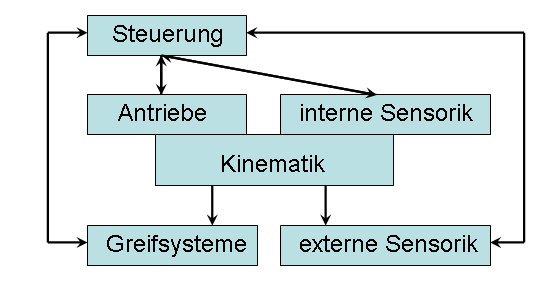
\includegraphics[width=0.6\textwidth]{images/stand_der_technik/Struktur_IR}
	\caption[Struktur eines Industrieroboters]{Struktur eines Industrieroboters \\Quelle: \cite{noauthor_industrieroboter_2020}}
	\label{fig:struktur_eines_industrieroboters}
\end{figure}
\FloatBarrier

Wie in Abbildung \ref{fig:struktur_eines_industrieroboters} zu sehen ist, besteht ein Industrieroboter grundlegend aus einem Roboterarm, welcher auch Manipulator genannt wird, einer Steuerungseinheit, welche für die Überwachungung und Übersetzung der Aktionen auf den spezifischen Industrieroboter zuständig ist und einem Effektor, welcher über ein Greifsystem befestigt wird. Über den Manipulator, welcher Gelenke und Antriebe aufweist, wird die Kinematik realisiert, welche es ermöglicht den Manipulator im Raum zu bewegen. Um jeden Punkt im 3D-Raum ansteuern zu können sind mindestens 3 DOF erforderlich, welche über Gelenke realisiert werden und translatorische oder rotatorische Bewegungen zulassen. Der Effektor kann auf verschiedene Arten realisiert werden. Zumeist ist es jedoch ein Werkzeug, welches z.B. für Schweiß-, Bohr- und Schneidearbeiten eingesetzt werden kann. Da der Effektor austauschbar ist, besteht jedoch aber auch die Möglichkeit einen Greifer oder einen anderen spezifisch für eine Aufgabe konzipierten Effektor zu montieren und zu verwenden. Damit die Steuerungseinheit die Gelenkpositionen und Antriebsgeschwindigkeiten ermitteln kann sind zudem Messsysteme erforderlich, welche als interne Sensoren bezeichnet werden. Als optionale Komponente können zudem externe Sensoren beim Industrieroboter verbaut sein, welche unter anderem zur Ermittlung von Objektposition im 3D-Raum und deren Größe verwendet werden können. Je nach Arbeitsumfeld kann es auch erforderlich sein, dass ein System zum Wechseln der Effektoren eingesetzt wird um mehrere Arbeitsschritte mit einem einzigen Industrieroboter durchführen zu können \cite{hagele_aufbau_2006}.




% https://de.wikipedia.org/wiki/Industrieroboter
% https://link.springer.com/chapter/10.1007%2F3-540-34823-9_27


% nach Kinematik unterschieden
% bestehen aus mehreren Gelenken
% serielle Roboter 95% & parallele 5% Roboter

% Arten & Vergleiche
% Genauigkeit
% Wie schnell können diese reagieren? (Zeitverhalten) je nach Roboterarm verschieden


\section{Arten von Teach Pendants}
% Arten von Handprogrammiergeräten
% Aufzählen
% Arten & Vergleiche
% Genauigkeit
% Wie funktioniert ein Teach Pendant
% Notaus stopp


\section{Arten von Zeitverhalten}
% Echtzeitverhalten
%    weiches & hartes Echtzeitverhalten
% Normales Zeitverhalten


\section{Sicherheitsanforderungen im Umgang mit Industrierobotern}


\section{ROS}
% Aufbauend auf dem Vergleich der Entwicklungsplattformen werden nun die für dieses Projekt am Besten geeigneten Werkzeuge vorgestellt.
% ROS 1 (LTS) vs ROS 2


\subsection{Architektur}


\subsection{Packages}


\subsection{Zukünftige Entwicklung}
% Community driven, ROS Foundation, ...


\subsection{Anbindungsmöglichkeiten/Interoperabilität}


\section{Simulations- und Testumgebungen}
% Gazebo, vRep, Coppelia Sim, ABB, ...


\section{Tiefensensoren}
% Arten und Vergleich (Vor- und Nachteile)
% Azure Kinect, ...
% Genauigkeit, Techniken, ...

\section{Positionsgenauigkeit}
%https://link.springer.com/chapter/10.1007%2F3-540-34823-9_27

\section{Gesten}
% Mögliche Gesten, Welche Gesten nicht


\section{Ergonomie}
